\documentclass[]{article}
\usepackage{amsfonts,amssymb,amsmath}
%\documentstyle[12pt,amsfonts]{article}
%\documentstyle{article}
\usepackage{biblatex}
\usepackage{graphicx}
\usepackage{listings}

\setlength{\topmargin}{-.5in}
\setlength{\oddsidemargin}{0 in}
\setlength{\evensidemargin}{0 in}
\setlength{\textwidth}{6.5truein}
\setlength{\textheight}{8.5truein}
\setcounter{MaxMatrixCols}{16}

\usepackage{color}

\definecolor{mygreen}{rgb}{0,0.6,0}
\definecolor{mygray}{rgb}{0.5,0.5,0.5}
\definecolor{mymauve}{rgb}{0.58,0,0.82}

\lstset{ %
  backgroundcolor=\color{white},   % choose the background color; you must add \usepackage{color} or \usepackage{xcolor}; should come as last argument
  basicstyle=\footnotesize,        % the size of the fonts that are used for the code
  breakatwhitespace=false,         % sets if automatic breaks should only happen at whitespace
  breaklines=true,                 % sets automatic line breaking
  captionpos=b,                    % sets the caption-position to bottom
  commentstyle=\color{mygreen},    % comment style
  deletekeywords={...},            % if you want to delete keywords from the given language
  escapeinside={\%*}{*)},          % if you want to add LaTeX within your code
  extendedchars=true,              % lets you use non-ASCII characters; for 8-bits encodings only, does not work with UTF-8
  frame=single,	                   % adds a frame around the code
  keepspaces=true,                 % keeps spaces in text, useful for keeping indentation of code (possibly needs columns=flexible)
  keywordstyle=\color{blue},       % keyword style
  language=Octave,                 % the language of the code
  morekeywords={*,...},           % if you want to add more keywords to the set
  numbers=left,                    % where to put the line-numbers; possible values are (none, left, right)
  numbersep=5pt,                   % how far the line-numbers are from the code
  numberstyle=\tiny\color{mygray}, % the style that is used for the line-numbers
  rulecolor=\color{black},         % if not set, the frame-color may be changed on line-breaks within not-black text (e.g. comments (green here))
  showspaces=false,                % show spaces everywhere adding particular underscores; it overrides 'showstringspaces'
  showstringspaces=false,          % underline spaces within strings only
  showtabs=false,                  % show tabs within strings adding particular underscores
  stepnumber=2,                    % the step between two line-numbers. If it's 1, each line will be numbered
  stringstyle=\color{mymauve},     % string literal style
  tabsize=2,	                   % sets default tabsize to 2 spaces
  title=\lstname                   % show the filename of files included with \lstinputlisting; also try caption instead of title
}

%\input ../basicmath/basicmathmac.tex
%
%\input ../adgeomcs/lamacb.tex
\input ./mac-new.tex
\input ./mathmac-v2.tex
%\input ../adgeomcs/mac.tex
%\input ../adgeomcs/mathmac.tex

\def\fseq#1#2{(#1_{#2})_{#2\geq 1}}
\def\fsseq#1#2#3{(#1_{#3(#2)})_{#2\geq 1}}
\def\qleq{\sqsubseteq}

%
\begin{document}

\title{CIS520 Report: ML Crackers}   % type title between braces
\author{Francine Leech, Ziyin Qu, Chen Xiang}         % type author(s) between braces
\date{December 12, 2016}    % type date between braces
\maketitle

\section{Introduction}

The rise in web and mobile based social networking has opened a stream of continuous text data. These data reflect the sentiment of individuals and masses of people. Understanding the sentiment of users is relevant on the most basic level, understanding how people are responding to a stimuli, and extending to human machine interaction systems. The ambiguity of language and emotional expression creates an interesting machine learning problem.  We try to tackle one aspect of this problem by classifying tweets into two categories, joy and sadness. 

\section{Preliminary Methods}

When starting the project, we thought that we should first experiment with different classification methods on image data like train\_color, train\_img\_prob because they were smaller datasets. Using our intuition we made the assumption that the image data contained basic information about people's sentiments. For example, lighter and bright colors represent joy, darker colors represent sadness. \\\\

Because the image data always contains a lot of features, so the method we use for image data is PCA and Gaussian Mixture Model. With PCA, we can reduce the dimensions of features, with GMM, if it works, we may cluster the training data into two clusters, joy and sadness and thus get the trained classifier. \\\\

For the training, we tried three datasets for PCA and GMM, that is train\_color, train\_img\_prob and train\_cnn\_feat. However, the results are not satisfying. The table below demonstrates the training accuracies with PCA and GMM on the three datasets.

\[
\begin{tabular}{|c|c|c|c|}
\hline &train\_color & train\_img\_prob & train\_cnn\_feat\\
\hline PCA and GMM&59\%&58\%&59\%\\
\hline
\end{tabular}
\]

We did not use cross validation for tuning the parameters because the training process will take a large amount of time and instead we used 4000 data to train and 500 hold out to test. We trained the image data in this way. We trained two GMM respectively for joy and sadness and each GMM has 5 clusters. For the PCA, we tried different numbers principle components for the three dataset but the results did not improve much.\\\\

We think the reason why PCA and GMM did not work on image data may because the image data itself does not contain enough information for this method to get a classifier, unlike other classical clustering problems like human face recognition or male and female recognition. The accuracy is not enough to beat the baseline 1, so we have to try different methods.

Dimensionality Reduction

We tried to reduce the dimensionality of the $word_train$ data using Principal Component Analysis to determine if we could classify the data with a PC-ed version of the training data using a Gaussian Mixture Model. We used a 'holdout' of 20\% of the train data to use as testing because cross validation with PCA took too long.  

$$Graph with PCA/GMM error/accuracy$$

Also, we found that using k nearest neighbors can't get good result and it is time consuming. Even if we use 10 fold cross validation and tried many similarity metrics, ended up with using spearman correlation and 449 neighbors. The accuracy is roughly 0.72, which is probably because the sparsity of data and the redundancy of attributes (the count of different words).
 


\section{Main Methods}

Here we describe the combination of models we used in our model. 


\subsection{Naive Bayes}

For supervised learning, Naive Bayes method is a very good generative method on classifying texts, like spam classification problem. Actually the words\_train data set uses bag of words model where counts of words matters and position of words does not matter. There are lots of advantages for Naive Bayes model, it can be a dependable baseline for text classification, it trains fast. Although the assumption of Naive Bayes which is the Conditional Independence Assumption may not be true, it may still work well on text classification problem.\\\\

To use the Naive Bayes model on words\_train dataset, we use the built-in matlab function fitNaiveBayes. For training data, we sue 9-fold cross validation error to estimate the test error for Naive Bayes model, which means we randomly choose 4000 data to train and 500 data to test. For the built-in function fitNaiveBayes, there are some parameters for us to choose, for the distribution parameter, because we are using the bag-of-words model, we use the multinomial distribution in the fitNaiveBayes function. \\\\

The Naive Bayes model actually works really well. We got around 0.8 cross validation accuracy on training data. And we got 0.7962 accuracy for the test data. We successfully beat the baseline1 using a simple Naive Bayes model with multinomial distribution. \\\\

But there are still problems with the simple Naive Bayes model. For example, the dataset matrix for words is very sparse, and for each observation there are many  words did not show up. Naive Bayes model for text assumes that there is no information in words that are not observed and this may cause over-fitting. We can solve this by smoothing the Naive Bayes model.

\subsection{GentleBoost}

The second main method we utilized was an ensemble method. We used GentleBoost, a weak learning that was built by MATLAB under the fitensemble function. The method combines many weak learners into one high quality ensemble predictor. We chose this ensemble methods over the others offered by MATLAB, because it is preforms well with binary classification trees with many predictors (ensemble citation). \\

The input of the model was the $word_train$ data. We used a 10-fold cross validation method to observed how the model preformed, specified the use 300 learners, and the type of learner as 'tree'. The average cross validation error was 0.21. The algorithm classified joy and sadness well. \\

The method could have improved if we increased the number of learners, however it would have taken a very long time to train because the data is large. Initially we tried the method with the default number of learners, 100 trees, and found that the cross validation accuracy only improved slightly. This slight improvement with triple number of learners reveals that the data has some intricacies or patterns that the ensemble method cannot learn.   


\subsection{Support Vector Machine}

Support vector machines (SVMs) proved to the most promising method to classify the data. We used the MATLAB function, fitcsvm, to train an SVM model for binary classification on the on the $word_train$ data.

We tried a simple SVM by specifying a linear kernel, and had a  cross validation error was 0.2180. With a Gaussian or RBF kernel we had an error of 0.4373. 


After experimenting with a variety of kernels, we found that the linear preformed the best. fitsvm allows you to make an assumption about the fraction of outliers in the data. While we could have gone through the raw tweets and looked through the data, we decided to experiment with  10\%, 20\%, and 30\% and observed cross validation errors 0.2121, 0.2282, and 0.2131 respectively. Specifying the outliers percentage did not have an effect on our cross validation error, so we decided not to specify in our SVM final model. 

Lastly we optimized our SVM by using MATLABs built in method to optimize a cross-validated SVM using Bayes Optimization (citation). The method originates from The Elements of Statistical Learning, Hastie, Tibshirani, and Friedman (2009). Paraphrasing from the MATLAB documentation,  "the model begins with generating 10 base points for a "green" class, distributed as 2D independent normals with mean (1,0) and unite variance. It then generates 10 base points for a "class" that is also distributed as 2-D independent normals with mean (0,1) and unit variance. For each of the classes, it generate 100 random points by choosing a base point, b, of the respective color uniformly at random. It then generates an independent random point with 2-D normal distribution with mean b and variance I/5, where I is the 2-by-2 identity matrix. After 100 points for each of the colors has been generated, the point are classified using fitcsvm. The function bayesopt is used to optimize the parameters of the final SVM model with respect to cross validation." We submitted the method to the autograder, and it had an accuracy of 0.7991. The method was accurate enough to beat Baseline 1, but not Baseline 2. Similar to the other methods above, the optimized SVM may not preform well because the data was sparse and high dimensional, so the hyperplane could not separate data well. 

\section{Final Method}

Our final method utilizes sentiment analysis, the classification of text into categories of emotions. We used the vaderSentiment 2.4.1 package in Python. VADER is a lexicon and rule-based sentiment analysis tool that is specifically attuned to sentiments expressed in social media. The advantage of this analysis is that we can use this preliminary method to discern extremely positive and extremely negative tweets by assuming that there are no extremely positive words shown in negative sentences and vise versa. We will describe the process of experimenting with two analyzes before selecting one to include in our final model. \\

\subsection{Sentiment Analysis 1}

In Python, we ran a sentimental analysis on each word present in the topwords\.csv. The input was each individual word in the list, and the output was the probability the word expresses a negative, positive, and neutral emotion. The output often looks like this, when type "funny" we can see \{'compound': 0.4404, 'neg': 0.0, 'neu': 0.0, 'pos': 1.0\}, which means it is an extremely positive word. \\


\subsection{Sentiment Analysis 2}

An issue we came across is from our first sentiment analysis is that we did not consider the raw tweets containing words that began with \#. These hash tags may represent the topic this sentence belongs to, some specific topics always express similar emotions, like \#family usually expresses a positive emotion. So instead of analyzing the sentiment of each word, we used sentence as the input and received the average emotion scores of each word.\\

We ran the sentimental analysis on each raw tweet using VADER package. For all the words that appeared in this sentence, we attached the resulting score to those words. For every word, an average emotion score is then based on all the raw tweets. \\ 

\subsection{Final Method}

Our final method which got 81.82\% accuracy on the leaderboard is achieved in this way. Firstly, from the testing on training dataset, we found that Sentiment Analysis has a high accuracy predicting those negative tweets. So the intuition was really straightforward, if the test data calculated by Sentiment Analysis 1 has negative words and don't have positive words, we will label it as negative. Then how we deal with those Sentiment Analysis can't predict? Because Naive Bayes and SVM and Gentleboost all have a quite good accuracy on test data, so we use the combine of the three methods through majority vote to predict them.\\\\
Figure 1 shows the structure of our final method. The majority vote goes in this way. We have three models predicting the test labels, if three of them all predict a tweet as sadness, we label this tweet as sad. If three of them all predict a tweet as joy, we will label them as joy. If any two of them predict a tweet as sadness, we label it as sadness. Finally if two of them predict a tweet as joy, we just use Naive Bayes results. Why in this situation we just use Naive Bayes instead of majority vote? Because the training accuracy tends to be higher for just use Naive Bayes in this situation than use majority vote.\\\\
Actually we also tried using Sentimental Analysis 2 with the combination of the three methods. But the accuracy did not improve. It may because the new Sentiment Analysis did not have that strong predictive words like Sentiment Analysis 1 has. Or maybe the result of Sentiment Analysis 1 is more suitable to the test data.


\begin{figure}
	\centering
  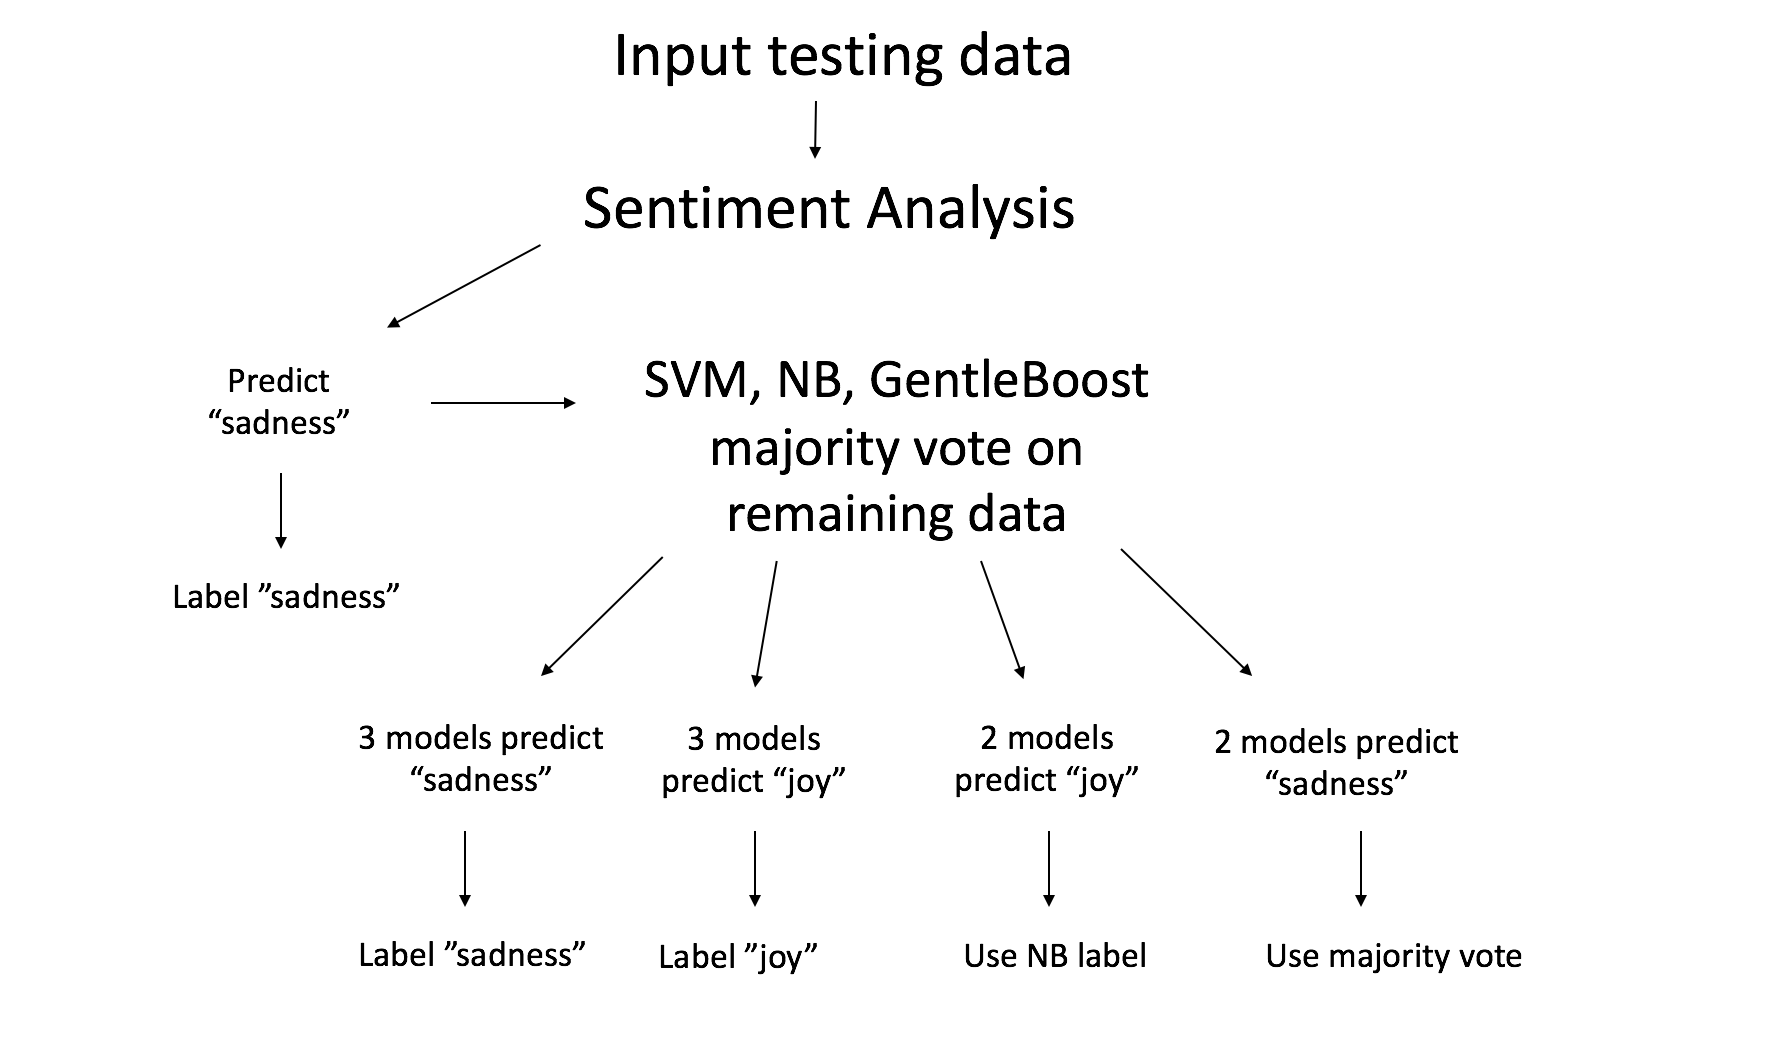
\includegraphics[scale=0.4]{Method.jpg}
  \caption{System Classification}
  \label{fig:System Classification}
\end{figure}

\begin{figure}
	\centering
  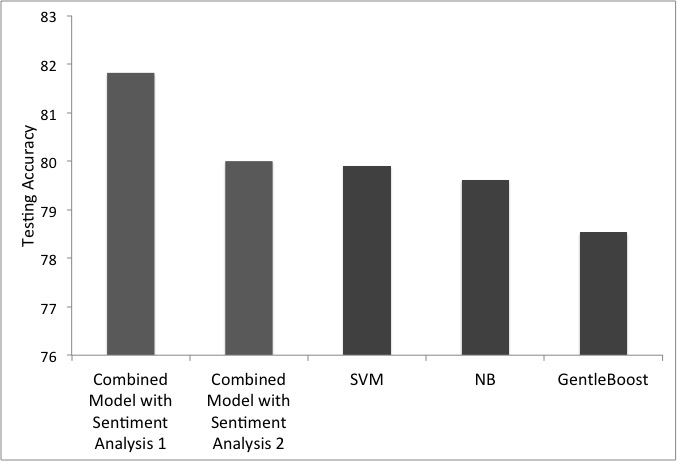
\includegraphics[scale=0.4]{FinalGraph.jpg}
  \caption{Test Error Final Models. The separate final models are in dark grey, and combined models with sentiment analysis are in light grey. The combined models have higher testing accuracy that the separate models. The combined model with sentiment analysis 2 preforms just as well as SVM. The model with Sentiment Analysis 1 has the highest testing accuracy.}
  \label{fig:Test Error}
\end{figure}

\section{Discussion}

Sentiment analysis is a difficult problem because human emotion is multifaceted and varies in intensity. In person, understanding the emotion a person is based on several parameters, the context of what they're saying, their words, tone, body language, and facial expression. Our classification problem is more difficult because we are given short tweets with a corresponding image. \\

One issue 
Issues with Lexicon
Developing the content of the lexicon is subjective. The use of language changes - how old is the lexicon being used? We don't know if the lexicon is comprehensive enough. Lexicon with emojis. 

What would our future method look like?
- Train classifier that train on emojis and hashtags since they are usually represent the topic of the tweet


Neutral tweets 


- Could have used deep learning 
	too long, overfit, dataset small
- articles \\
Other methods we tried on words includes TF-IDF. TF-IDF is short for term frequency–inverse document frequency, is a numerical statistic that is intended to reflect how important a word is to a document in a collection or corpus. It is often used as a weighting factor in information retrieval and text mining. We use this method to transform the train data and then use SVM or logistic regression methods to predict. However, the results are not satisfying. It may because the training data are too sparse and many of them didn't show up, so the result of TF-IDF can not give us more information about the train set.

\section{Works Cited}
\begin{thebibliography}{1}

%\bibitem{ensemble} Documentation. Ensemble Methods - MATLAB & Simulink. N.p., n.d. Web. 11 Dec. 2016. 

\end{thebibliography}

\section{Appendix}

\lstinputlisting[language=Python]{"./sentimental analysis with python.py"}





\end{document}
